\documentclass[12pt,a4paper]{article}
\usepackage[utf8]{inputenc}
\usepackage{amsmath}
\newcommand{\norm}[1]{\left\lVert#1\right\rVert}
\usepackage{amsfonts}
\usepackage{comment}
\usepackage{nicefrac}
%\usepackage[margin=2cm]{geometry}
\usepackage{amssymb}
\usepackage{accents}
\usepackage{amsthm}
\usepackage[pdftex, pdfborderstyle={/S/U/W 0}]{hyperref}
\numberwithin{equation}{section}
\usepackage{commath}
\usepackage[italian]{babel}
\usepackage{graphicx}
%\usepackage[extreme]{savetrees}
\usepackage{bm}
\usepackage{indentfirst}

\usepackage{cool}
\Style{DSymb={\mathrm d},DShorten=true,IntegrateDifferentialDSymb=\mathrm{d}}

\usepackage{microtype}
\usepackage{cleveref}

\usepackage{url}
\newcommand*{\defeq}{\stackrel{\text{def}}{=}}
\author{Jacopo Tissino \\
VB
(CLIL)\\
Liceo Scientifico M. Grigoletti}
\date{A. S. 2015--16}
\title{\huge{\textbf{Turbolenza}}\\
\Large{Fluidodinamica e Van Gogh}}
\begin{document}

\maketitle

\begin{abstract}
Partiamo da una trattazione delle equazioni di Navier-Stokes (per un fluido non comprimibile, ignorando le forze esterne), per poi capire cos'è il regime turbolento e quali sono le basi della teoria proposta da Kolmogorov nel 1941.

Così, arriviamo allo studio \cite{study2006}, che applica questa teoria (invece che alla velocità di un fluido) alla luminanza dei quadri di Van Gogh, trovando degli interessanti collegamenti.
\end{abstract}

\begin{figure}[h]
    \centering
    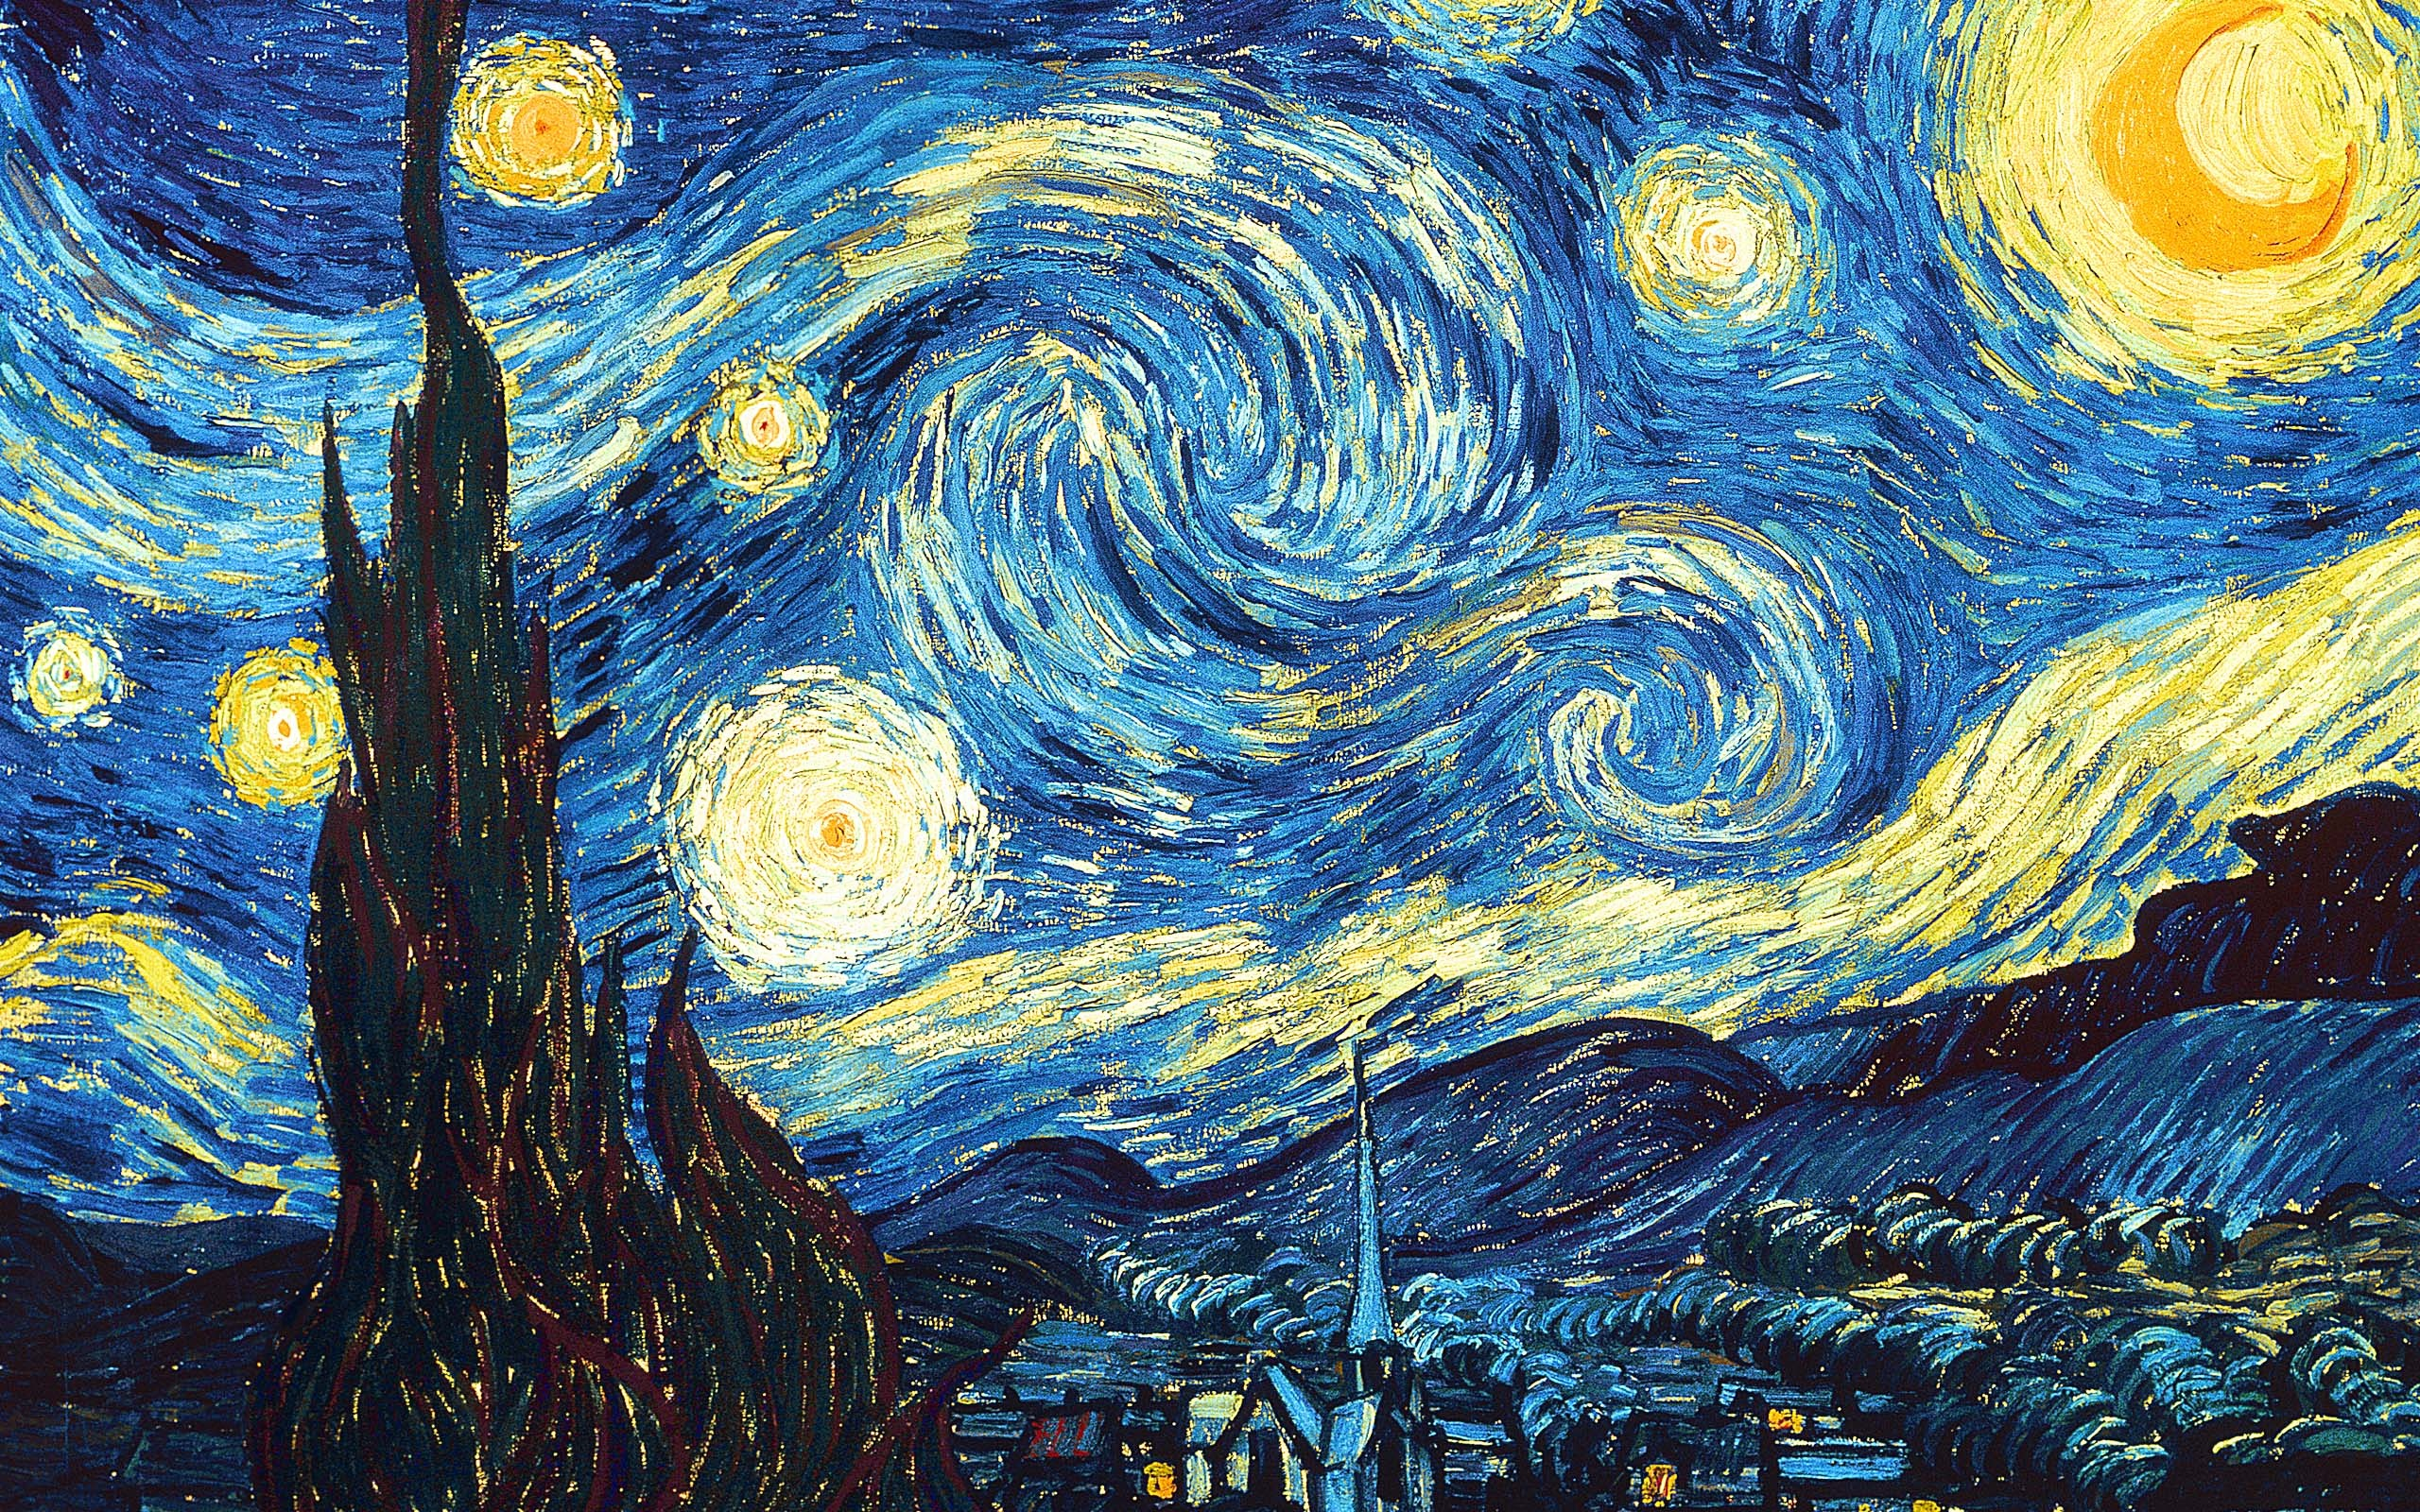
\includegraphics[scale=0.15]{the-starry-night-1889.jpg}
    \caption{\emph{Notte Stellata}.}
    \label{starrynight}
\end{figure}

\begin{figure}
    \centering
    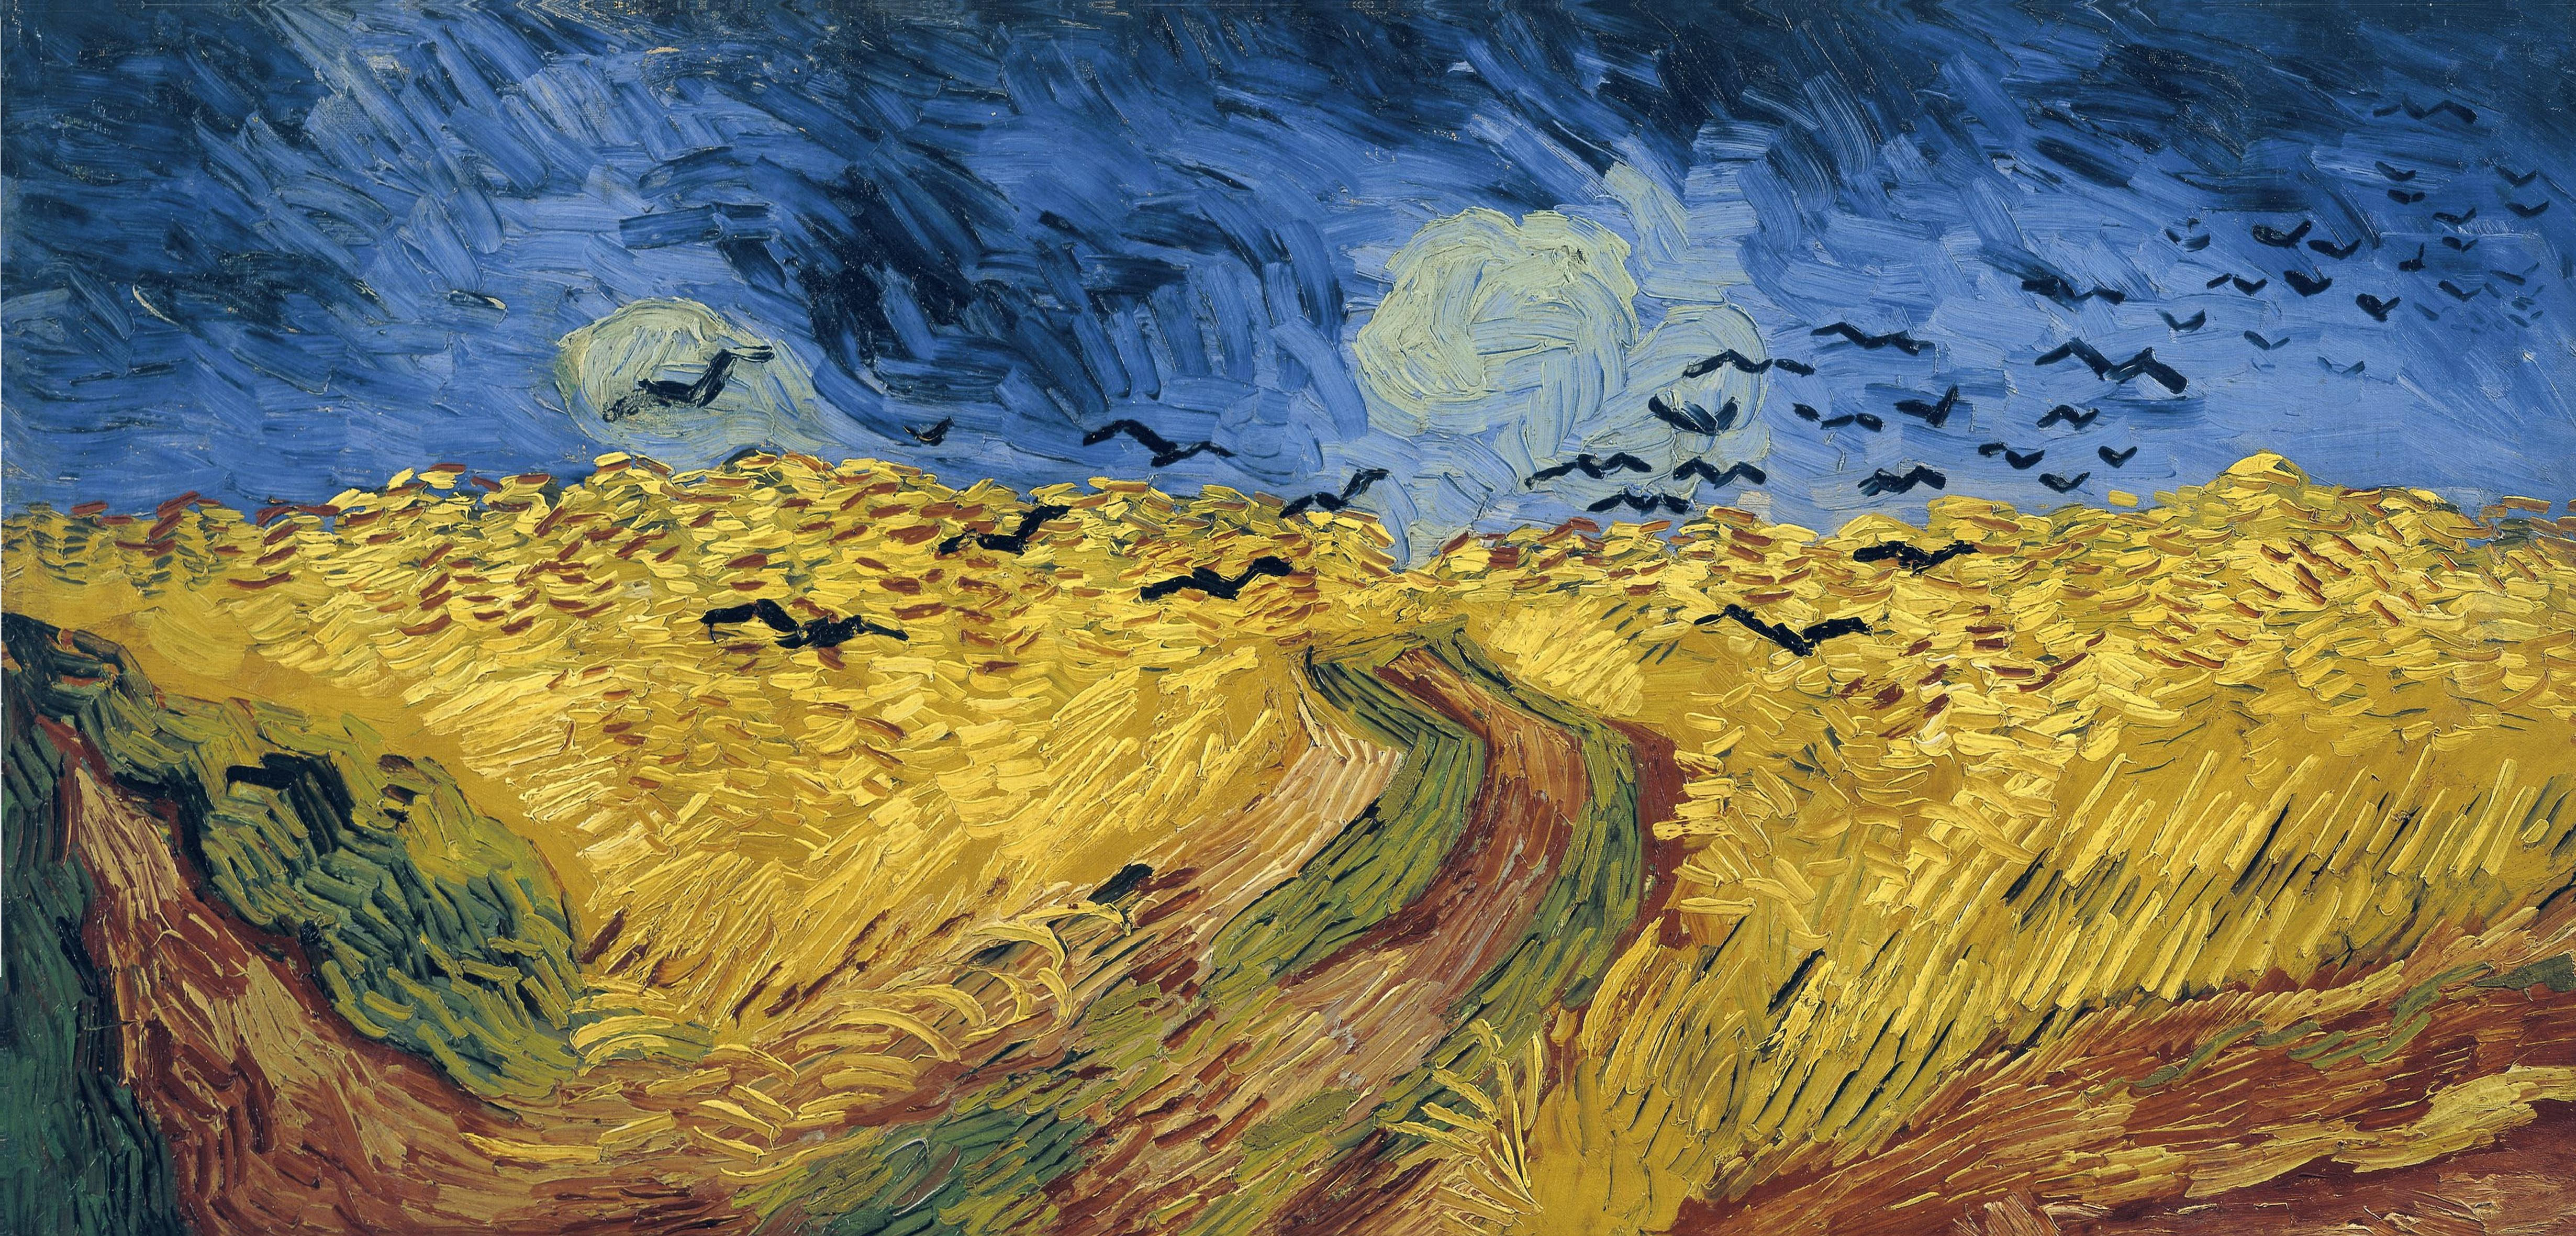
\includegraphics[scale=0.12]{wheatfield.jpg}
    \caption{\emph{Wheatfield with crows}.}
    \label{wheatfield}
\end{figure}

\begin{figure}
    \centering
    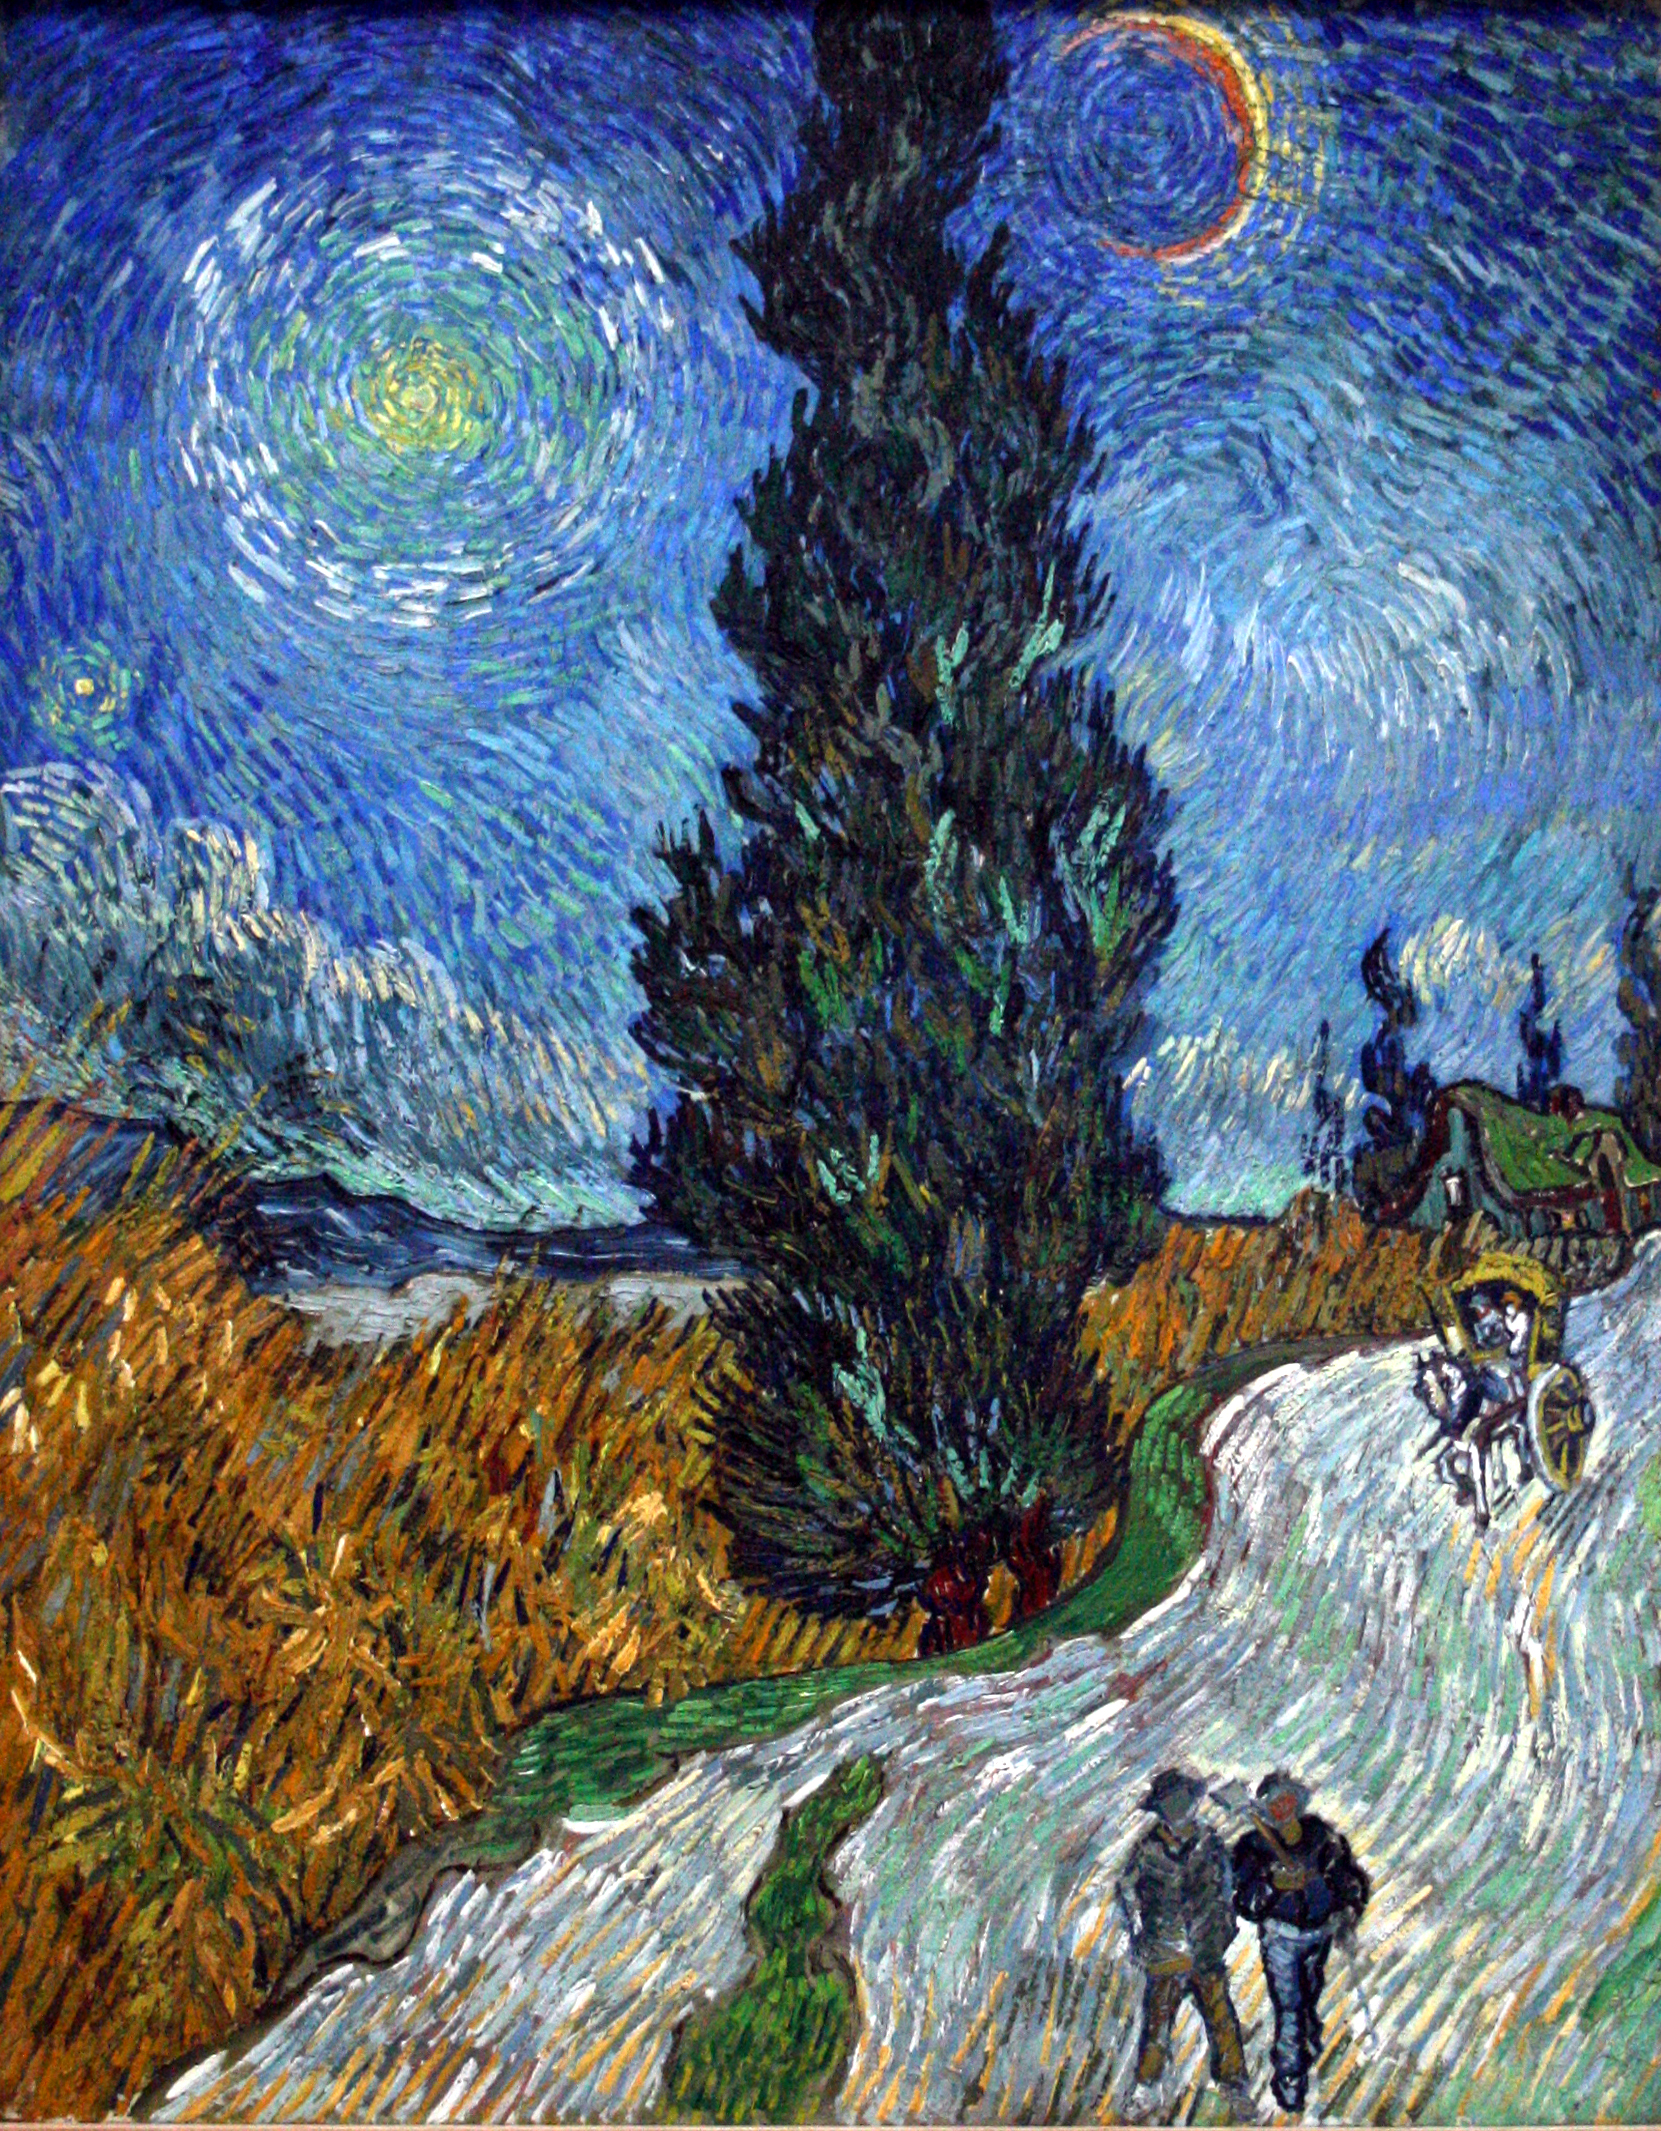
\includegraphics[scale=0.12]{road_cypress.jpg}
    \caption{\emph{Road with cypress and star}.}
    \label{road}
\end{figure}

\section{Navier-Stokes}

\subsection{Ricavarle}

Partiamo \cite{derivationns} dal \emph{teorema del trasporto di Reynolds}, che afferma qualcosa di apparentemente scontato: data una certa proprietà intensiva (che può essere anche vettoriale) di una sostanza in un volume, la variazione dell'integrale di questa proprietà nel volume sarà pari alla differenza fra quanta ne entra e quanta ne esce, sommata a quanta proprietà si genera o si distrugge nel volume.

Se il nostro volume è $\Omega$, la proprietà intensiva è $\phi$, il suo flusso è $\mathbf{v}$, e $s$ sono le \emph{sources}, ovvero i luoghi dove la proprietà viene generata, scriviamo:

\begin{equation}
\frac{\text{d}}{\text{d} t} \iiint_{\Omega} \phi \, \text{d} V = -
\iint_{\partial \Omega} \phi \mathbf{v} \cdot \mathbf{\hat{n}} \, \text{d} A +
\iiint_{\Omega} \mathbf{s} \, \text{d} V
\end{equation}

Applicando il teorema della divergenza, possiamo rendere tutti gli integrali volumetrici, poi portare la derivata temporale nel primo integrale secondo la regola di Leibniz, per ottenere:\\*
\begin{equation}
\frac{\partial \phi}{\partial t} = - \nabla \cdot ( \phi \mathbf{v} ) + \mathbf{s}
\end{equation}

\paragraph{Massa}

Se applichiamo il teorema del trasporto di Reynolds alla densità  --- ovvero scegliamo come proprietà generica $\phi$ la densità $\rho$, definita in modo tale che per un volume $\Omega$ la massa $m$ sia pari a

\begin{equation}
m = \iiint_{\Omega} \rho \dif V
\end{equation}

--- per la conservazione della massa abbiamo $\mathbf{s} = 0$ (non esistono ``generatori'' di massa),  otteniamo:

\begin{equation}
\frac{\partial \rho}{\partial t} + \nabla \cdot ( \rho \mathbf{v} ) = 0 \label{consmassa}
\end{equation}

Postulando che il fluido non possa essere compresso --- ovvero che la densità sia costante nel tempo e nello spazio, in formule $\frac{\text{d} \rho}{\text{d} t} = 0$ e $\nabla \rho = 0$, in quanto una variazione della densità del fluido nel tempo implicherebbe che questo si è compresso o espanso --- ricaviamo:\\*
\begin{equation}
\nabla \cdot \mathbf{v} = 0
\end{equation}

\paragraph{Quantità di moto}

Se, invece, applichiamo il teorema alla quantità di moto (sostituiamo alla generica proprietà intensiva $\phi$  il vettore $\rho \mathbf{v}$), ricaviamo:

\begin{equation}
\pderiv{(\rho \mathbf{v})}{t} + \nabla \cdot ( \rho \mathbf{v} \mathbf{v} ) =  \mathbf{s}
\end{equation}

dove con abuso di notazione intendiamo per $\mathbf{v} \mathbf{v}$:

\begin{equation}
\mathbf{v} \mathbf{v} = (v_i v_j)\mathbf{e}_i \otimes \mathbf{e}_j = \begin{pmatrix}
v_x v_x & v_x v_y & v_x v_z \\
v_y v_x & v_y v_y & v_y v_z \\
v_z v_x & v_z v_y & v_z v_z 
\end{pmatrix} \label{vettorepervettore}
\end{equation}

dove per $\mathbf{e}_i$ intendiamo un versore nell'$i$-esima direzione.

Compare dunque la divergenza di un tensore: questa è definita come il vettore

\begin{equation}
\nabla \cdot \mathbf{T} = \left( \sum_{i} \frac{\partial T_{ij}}{\partial x_i} \right) \mathbf{e}_j\end{equation}

(spesso si omette la somma).

Semplifichiamo dunque, utilizzando le seguenti identità dell'analisi tensoriale: \\*
\begin{itemize}
\item $\nabla \cdot (\phi \mathbf{A}) = \mathbf{A} (\nabla \phi) + \phi (\nabla \cdot \mathbf{A})$ 
\item $\nabla \cdot (\mathbf{A} \mathbf{B}) = \mathbf{A} \cdot (\nabla \mathbf{B}) + (\nabla \mathbf{A})\cdot \mathbf{B}$.
\end{itemize}

\begin{align}
\rho \pderiv{\mathbf{v}}{t} + \mathbf{v}\pderiv{\rho}{t} + \mathbf{v} \mathbf{v} \cdot \nabla \rho
+ \rho \left( \mathbf{v} \cdot (\nabla \mathbf{v}) + \mathbf{v} (\nabla \cdot \mathbf{v})  \right) &= \mathbf{s} \nonumber \\
\mathbf{v}\left( \pderiv{\rho}{t} + \mathbf{v} \cdot \nabla \rho + \rho (\nabla \cdot \mathbf{v}) \right) + \rho \left( \pderiv{\mathbf{v}}{t} + \mathbf{v} \cdot (\nabla \mathbf{v}) \right) &= \mathbf{s} \nonumber \\
\mathbf{v}\left( \pderiv{\rho}{t} + \nabla \cdot (\rho \mathbf{v}) \right) + \rho \left( \pderiv{\mathbf{v}}{t} + \mathbf{v} \cdot (\nabla \mathbf{v}) \right) &= \mathbf{s} \label{qdm}
\end{align}

Per la \eqref{consmassa} il termine moltiplicato per $\mathbf{v}$ nella \eqref{qdm} è pari a 0, dunque ci rimane:

\begin{equation}
\rho \left( \pderiv{\mathbf{v}}{t} + \mathbf{v} \cdot (\nabla \mathbf{v}) \right) = \mathbf{s}
\end{equation}

L'integrale volumetrico del termine $\mathbf{s}$ comprende tutti gli altri tipi di forze che possono agire sull'infinitesimo di volume.

\begin{figure}
    \centering
    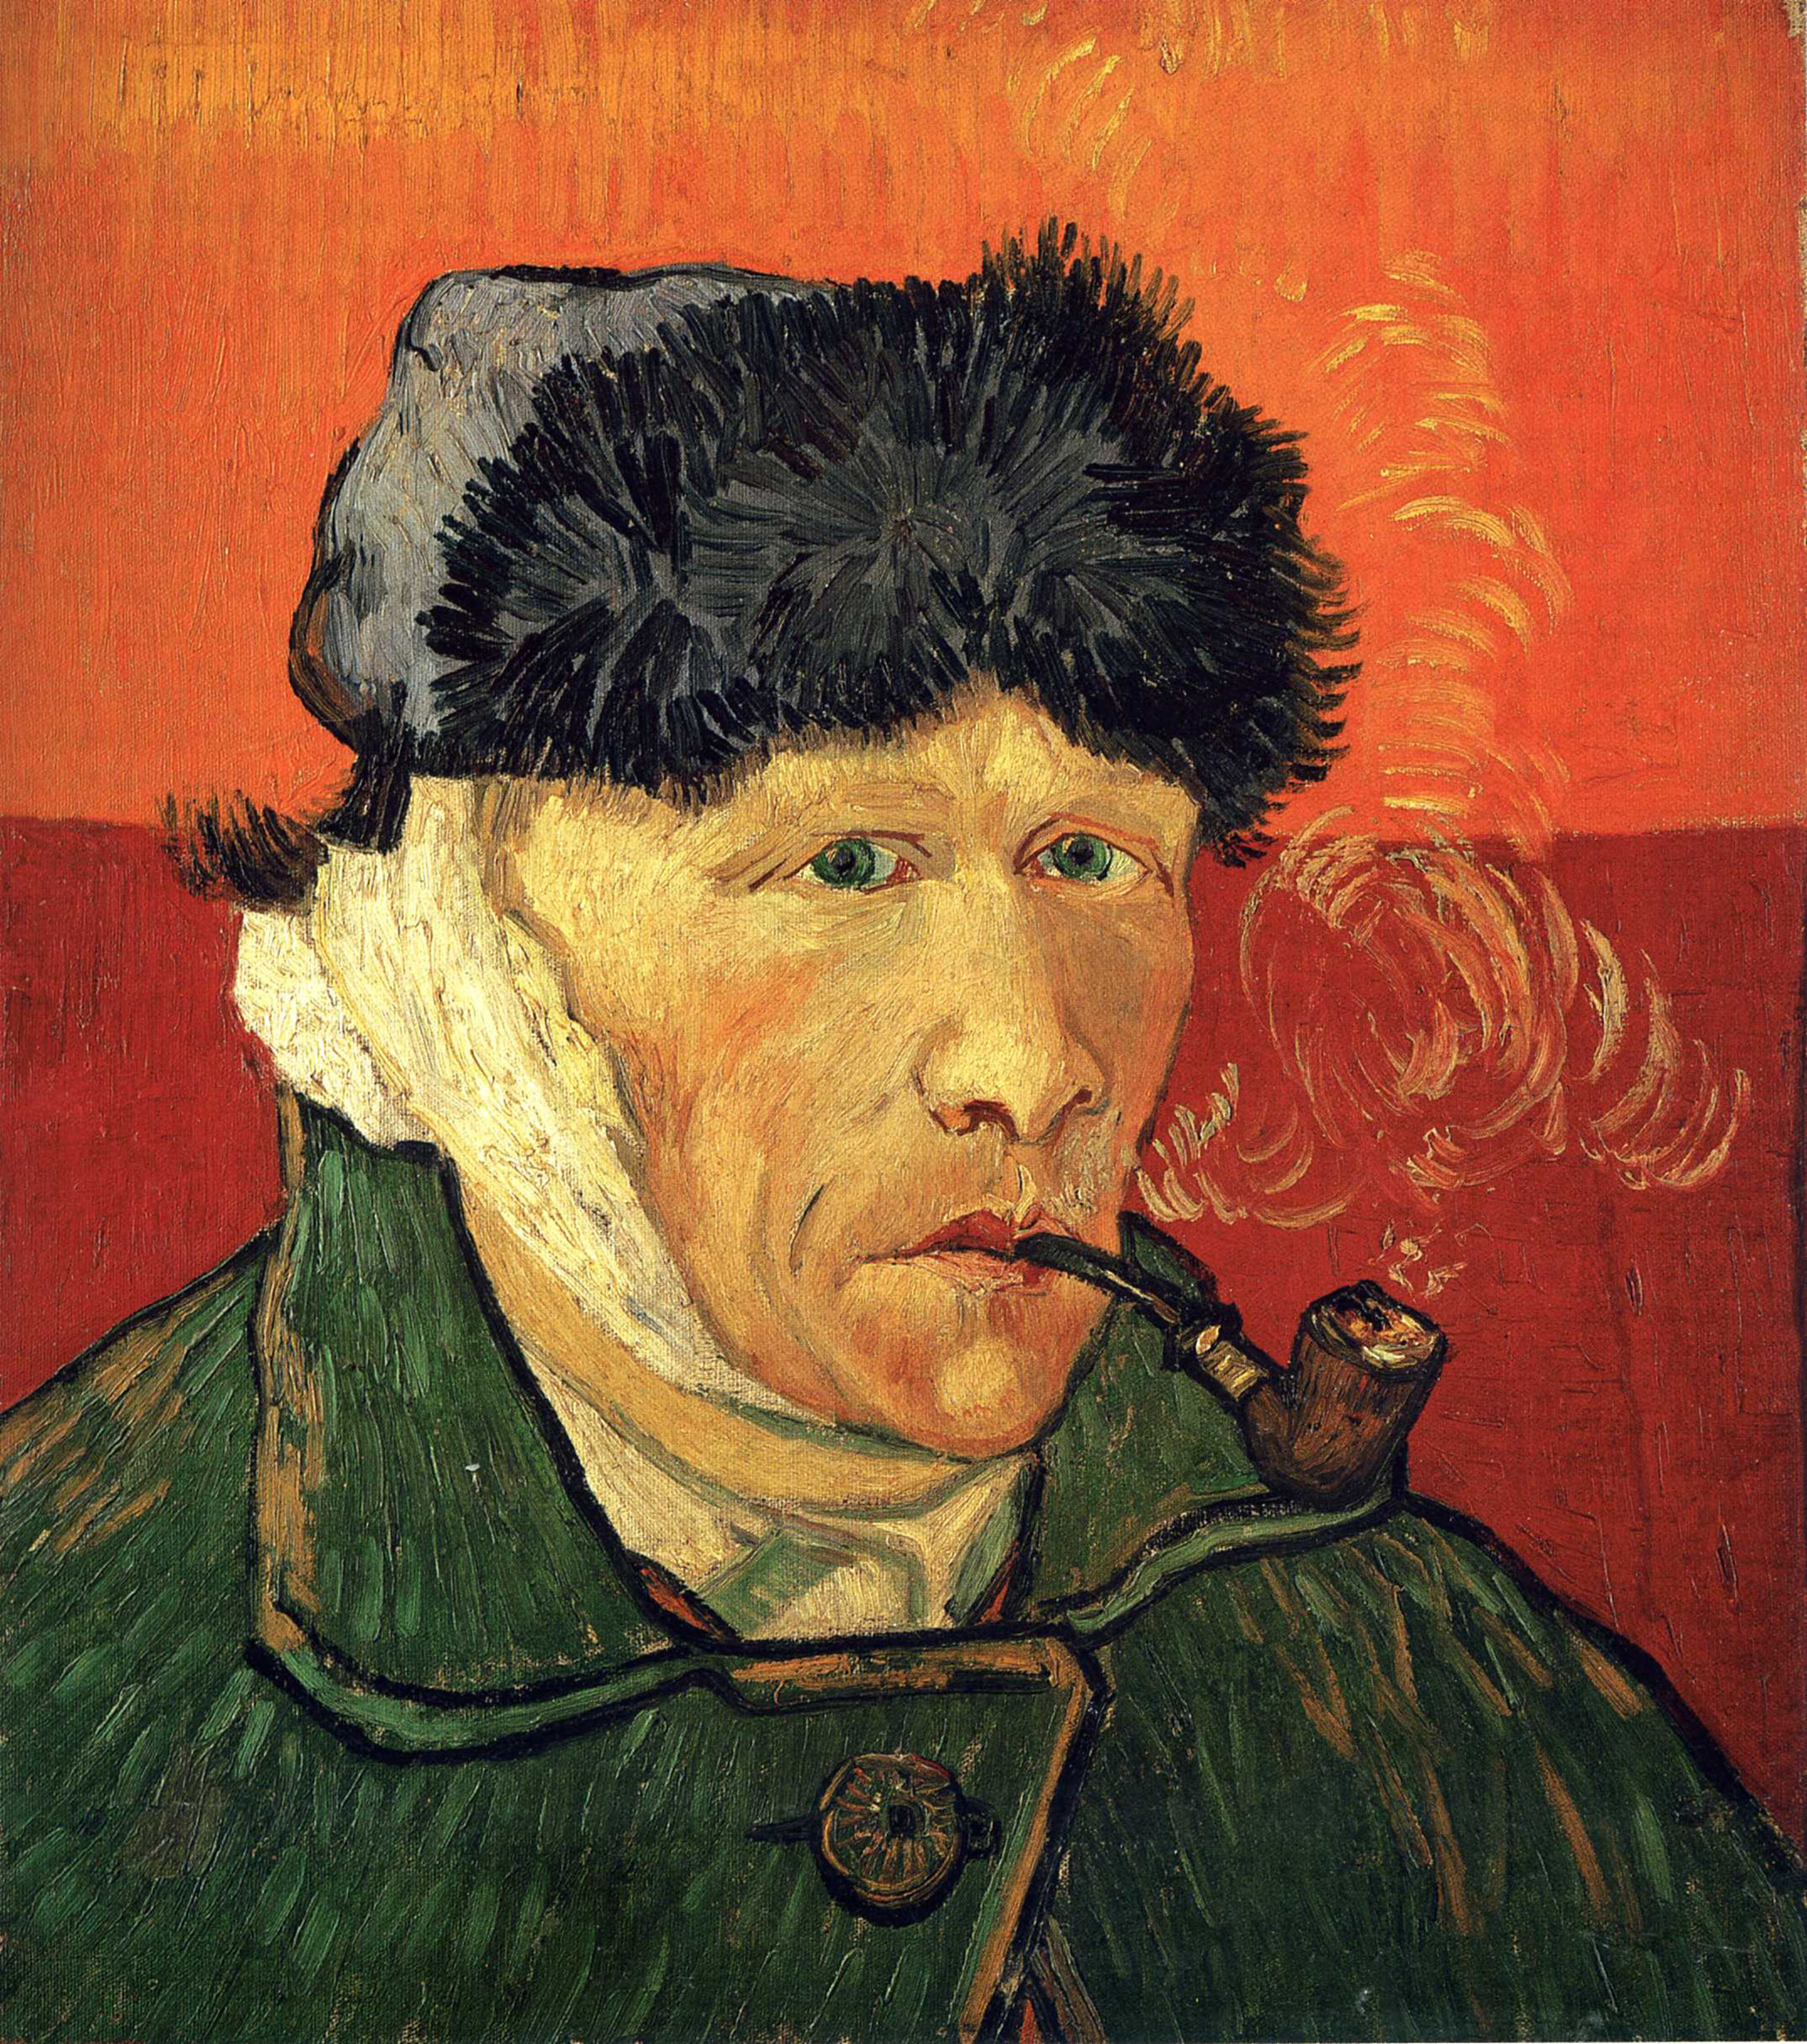
\includegraphics[scale=0.10]{selfportrait.jpg}
    \caption{\emph{Self-portrait with pipe and bandaged ear}.}
    \label{self}
\end{figure}

Ignorando le \emph{body forces} (come la gravità), possiamo scrivere

\begin{equation}
\mathbf{s} = \nabla \cdot \bm{\sigma}
\end{equation}

Dove $\bm{\sigma}$ è un tensore del secondo ordine che include tutti gli sforzi sull'infinitesimo di volume $\mathrm{d}V$. 

\begin{equation}
\bm{\sigma} = \begin{pmatrix}
\sigma_{xx} &  \tau_{xy} & \tau_{xz} \\
\tau_{yx} &  \sigma_{yy} & \tau_{yz} \\
\tau_{zx} &  \tau_{zy} & \sigma_{zz}
\end{pmatrix}
\end{equation}

Lo possiamo dividere in pressione e forze viscose, ovvero consideriamo prima le componenti ortogonali e poi gli sforzi di taglio.

Scomponiamo quindi $\bm{\sigma}$ in:\\*
\begin{equation}
\bm{\sigma} = -p I_3 + \begin{pmatrix}
\sigma_{xx} + p &  \tau_{xy} & \tau_{xz} \\
\tau_{yx} &  \sigma_{yy} + p & \tau_{yz} \\
\tau_{zx} &  \tau_{zy} & \sigma_{zz} + p
\end{pmatrix}
\end{equation}

dove  $I_3$ è una matrice identità tre per tre. Se definiamo la pressione come un meno un terzo della traccia di $\bm{\sigma}$ (possiamo farlo assumendo che il flusso sia isotropico), ci rimane $\bm{\sigma} = -p I_3 + \bm{\tau}$. Intuitivamente, il primo termine rappresenta le forze che cercano di comprimere il parallelepipedo, mentre il secondo quelle che tendono a distorcerlo.

Dunque, la forma dell'equazione per ora è:

\begin{equation}
\mathbf{s} = - \nabla p + \nabla \cdot \bm{\tau}
\end{equation}

\subparagraph{Forza viscosa}

Consideriamo una sola direzione del parallelepipedo $\mathrm{d} V$, ovvero due faccie parallele. Se il fluido che consideriamo è newtoniano, è stato osservato che:

\begin{equation}
\tau_{ij} = \mu 
    \left( 
        \pderiv{v_i}{x_j} + 
        \pderiv{v_j}{x_i}
    \right) \label{fvisc}
\end{equation}

dove $\mu$ è la cosiddetta \emph{viscosità dinamica}.

Troviamo poi che:

\begin{equation}
\nabla \cdot \bm{\tau} =
    \pderiv{\tau_{ij}}{x_i}\mathbf{e}_j =
    \mu \left(
        \frac{\partial}{\partial x_i}        
        \left(
            \pderiv{v_i}{x_j}+
            \pderiv{v_j}{x_i}+
        \right)        
        \mathbf{e}_j
    \right) 
\end{equation}

e ricordando che per la conservazione della massa $\nabla \cdot \mathbf{v} = 0$ arriviamo a:

\begin{equation}
\nabla \cdot \bm{\tau} = \mu \nabla ^2 \mathbf{v}
\end{equation}

\subsection{Formulazione}

Sinteticamente, dunque, le equazioni di Navier-Stokes si possono esprimere così:

\begin{subequations}
\begin{align}
\frac{\partial \mathbf{v}}{\partial t} + \mathbf{v} \cdot (\nabla \mathbf{v})  &= -\frac{\nabla p}{\rho} + \nu \nabla^2 \mathbf{v} \label{navier-stokes} \\
\nabla \cdot \mathbf{v} &= 0
\end{align}
\end{subequations}

Possiamo introdurre l'operatore $\Dif / \Dif t$:

\begin{equation}
\frac{\Dif \mathbf{a}}{\Dif t} =
\pderiv{\mathbf{a}}{t} + \mathbf{v} \cdot (\nabla \mathbf{a}) 
\end{equation}

Oppure, scrivendo tutte le derivate parziali esplicitamente, se il vettore velocità è $\mathbf{v} (u, v, w)$:

\renewcommand{\arraystretch}{2}
\begin{equation}
\frac{\partial}{\partial t} \begin{bmatrix}
u \\
v \\
w 
\end{bmatrix} +
\begin{bmatrix}
u \dfrac{\partial u}{\partial x} & v \dfrac{\partial u}{\partial y} & w \dfrac{\partial u}{\partial z} \\
u \dfrac{\partial v}{\partial x} & v \dfrac{\partial v}{\partial y} & w \dfrac{\partial v}{\partial z} \\
u \dfrac{\partial w}{\partial x} & v \dfrac{\partial w}{\partial y} & w \dfrac{\partial w}{\partial z} \\
\end{bmatrix} =
-\dfrac{1}{\rho}
\begin{bmatrix}
\dfrac{\partial p}{\partial x} \\
\dfrac{\partial p}{\partial y} \\
\dfrac{\partial p}{\partial z} \\
\end{bmatrix} +
\nu 
\begin{bmatrix}
\dfrac{\partial^2 u}{\partial x^2} & \dfrac{\partial^2 u}{\partial y^2} & \dfrac{\partial^2 u}{\partial z^2} \\
\dfrac{\partial^2 v}{\partial x^2} & \dfrac{\partial^2 v}{\partial y^2} & \dfrac{\partial^2 v}{\partial z^2} \\
\dfrac{\partial^2 w}{\partial x^2} & \dfrac{\partial^2 w}{\partial y^2} & \dfrac{\partial^2 w}{\partial z^2} \\
\end{bmatrix}
\end{equation}

\subsection{Il numero di Reynolds}

È definito come

\begin{equation}
\text{Re} = \frac{v L}{\nu} = \frac{\rho v L}{\mu}
\end{equation}

dove $v$ è la velocità media del flusso e $L$ è la lunghezza caratteristica del tratto che consideriamo.
Rappresenta il rapporto fra le forze inerziali e quelle viscose: infatti, scegliendo un volume (come un cilindro) di superficie $S$ e lunghezza $L$, e un tempo unitario $t$ (interpretando dunque le derivate come semplici divisioni per tale intervallo) possiamo esprimerle come

\begin{subequations}
\begin{align}
F_i = m a = \rho S L \frac{L}{t^2}\\
F_v = \mu S \frac{\Delta v}{\Delta L} = \frac{\mu S L}{Lt}
\end{align}
\end{subequations}

da cui

\begin{equation}
\text{Re} = \frac{F_i}{F_v} =  \frac{\rho L^2}{t \mu} = \frac{\rho L v}{\mu}
\end{equation}

\paragraph{Ricaviamolo}

Prendiamo la \eqref{navier-stokes} e moltiplichiamola per $L/v^2$, dove $L$ è una lunghezza caratteristica e $v$ è la velocità media.

Ridefiniamo poi: 

\begin{equation}
\mathbf{v'} = \frac{\mathbf{v}}{v},\qquad p' = \frac{p}{\rho v^2},\qquad \frac{\partial}{\partial t'} = \frac{L}{v} \frac{\partial}{\partial t},\qquad \nabla' = L \nabla
\end{equation}

Ricaviamo dunque l'equazione adimensionalizzata: 

\begin{equation}
\frac{\partial \mathbf{v'}}{\partial t'} +\mathbf{v'} \cdot (\nabla' \mathbf{v'})  = -\nabla' p' + \frac{\mu}{\rho L v} \nabla'^2 \mathbf{v'}
\end{equation}

Ovvero, togliendo i primi:

\begin{equation}
\frac{\partial \mathbf{v}}{\partial t} +\mathbf{v} \cdot (\nabla \mathbf{v}) = -\nabla p + \frac{1}{\text{Re}} \nabla^2 \mathbf{v}
\end{equation}

Si può dunque vedere che, al tendere di Re all'infinito, il termine viscoso scompare, rendendo il regime completamente inerziale.

\paragraph{Valutazioni qualitative}

\begin{itemize}
\item Ad alti numeri di Reynolds, le forze inerziali dominano e il regime è \emph{turbolento}, mentre
\item a bassi numeri di Reynolds, le forze viscose dominano e il regime è \emph{laminare}.
\end{itemize}

\section{Il flusso turbolento}

Quando il moto diventa turbolento, a quello principale della direzione della velocità media si sovrappongono moti secondari in direzioni perpendicolari, che provocano rimescolamento e vortici \cite{dispense}.

Dividiamo la velocità in una parte media e una fluttuazione: $\mathbf{v} = \mathbf{\overline{v}} + \mathbf{v'}$, dove $\mathbf{v'}$ è la fluttuazione, ovvero $\mathbf{\overline{v'}} =  0$, e facciamo lo stesso per la pressione ($p = \overline{p} + p'$).

Per media $\overline{\varphi}$ di una quantità qualsiasi $\varphi (t)$ in un punto fisso dello spazio, intendiamo:

\begin{equation}
\overline{\varphi} = \frac{1}{\vartheta} \int^{t_0 + \vartheta}_{0} \varphi \, \text{d}t
\end{equation}

Applicando le proprietà della media, possiamo ricavare la versione \emph{mediata} delle equazioni di Navier-Stokes:

\begin{subequations}
\begin{align}
\frac{\Dif \mathbf{\overline{v}}}{\Dif t}   &= -\frac{\nabla \overline{p}}{\rho} + \nu \nabla^2 \mathbf{\overline{v}} - \nabla \cdot \left(
\overline{\mathbf{v'}\mathbf{v'}}
\right)\\
\nabla \cdot \mathbf{\overline{v}} &= 0
\end{align}
\end{subequations}

dove $\overline{\mathbf{v'}\mathbf{v'}}$ è sempre un tensore, secondo la formula \eqref{vettorepervettore}.

\paragraph{Viscosità turbolenta}

Consideriamo il tensore $\overline{\mathbf{v'}\mathbf{v'}} = \bm{\sigma}_T$ come parte di $\bm{\tau}$, il tensore che prima abbiamo considerato come componente viscosa, ovvero assimiliamo gli effetti della turbolenza ad un incremento della viscosità (non reale, ma efficace).

Se prima avevamo trovato la \eqref{fvisc}, sperimentalmente è stato anche ricavato:

\begin{equation}
\sigma_{Tij} = - \rho \overline{v'_i v'_j} = \mu_t \left(
\pderiv{\overline{v_i}}{x_j} + \pderiv{\overline{v_j}}{x_i}
\right)
\end{equation}

Dove $\mu_T$, la \emph{viscosità turbolenta}, non è una proprietà del fluido ma  dipende dallo stato della turbolenza.

L'equazione di conservazione della quantità di moto si trasforma quindi in:

\begin{equation}
\frac{\Dif \mathbf{\overline{v}}}{\Dif t}  = -\frac{\nabla \overline{p}}{\rho} + (\nu + \nu_T ) \nabla^2 \mathbf{\overline{v}} 
\end{equation}

dove chiaramente $\nu_T = \mu_T / \rho$

\subsection{La teoria di Kolmogorov}

Il flusso turbolento è composto da vortici di diverse dimensioni. L'energia viene trasmessa dai più grandi ai più piccoli, fino a quando non viene dissipata completamente dalla frizione viscosa. Questo è stato espresso dal poeta Lewis Fry Richardson:

\begin{verse}
Big whorls have little whorls, \\
which feed on their velocity; \\
And little whorls have lesser whorls, \\
And so on to viscosity. \cite{richardson}
\end{verse}


Chiamiamo $d$ dimensione del vortice e $\accentset{\circ}{v}$ la sua velocità orbitale: osserviamo che la seconda è funzione della prima ($\accentset{\circ}{v} = f(d)$).

\paragraph{Tasso di dissipazione}

Il \emph{tasso di dissipazione} $\epsilon$ è definito come 

\begin{equation}
\epsilon = \frac{\text{energia convertita in calore}}{\text{massa unitaria} \times \text{tempo unitario}}
\end{equation}

Il fatto che la turbolenza sia statisticamente omogenea implica che i passaggi di energia da una scala ad un'altra siano uguali: l'energia inizialmente fornita ai vortici più grandi è pari a quella passata a quelli più piccoli, e infine a quella dissipata in calore.
Dunque, malgrado il comportamento sia sempre caotico, possiamo dire che il comportamento dei grandi vortici è simile a quello dei più piccoli.

Come dimensioni:

\begin{equation}
[\epsilon ] = L^2 T^{-3}
\end{equation}

Assumiamo che $\accentset{\circ}{v} \propto (\epsilon d)^k$. Dimensionalmente, otteniamo:

\begin{equation}
\accentset{\circ}{v} = A (\epsilon d)^{1/3} \label{scaling}
\end{equation}

dove $A$ è una costante adimensionale.

La turbolenza avviene fra $d_{\text{max}}$ e $d_{\text{min}}$. La prima è la dimensione del sistema, la seconda invece è la scala alla quale avviene la dissipazione in calore, e Kolmogorov ha postulato che dipenda solo da $\epsilon$ e $\nu$. Dimensionalmente:

\begin{equation}
d_{\text{min}} \sim \nu^{3/4} \epsilon^{-1/4}
\end{equation}

$\nu^{3/4} \epsilon^{-1/4}$ = scala di Kolmogorov

\begin{comment}

\subsection{Spettro di energia}

Definiamo il \emph{numero d'onda} come:

\begin{equation}
k = \frac{\pi}{d}
\end{equation}

(non $2\pi$ perché la velocità cambia verso se passiamo da una parte all'altra del vortice)

$k_{\text{min}} = \pi / d_{\text{max}}$, $k_{\text{max}} \sim \nu^{-3/4} \epsilon^{1/4}$

$E_k$ è l'energia cinetica per massa di fluido, con dimensioni $L^2 T^{-2}$

\begin{equation}
\dif E = E_k (k) \dif k
\end{equation}

Dimensionalmente:

\begin{equation}
E_k (k) = B \epsilon^{2/3} k^{-5/3}
\end{equation}

\begin{equation}
\int^{\infty}_{k_{\text{min}}} E_k (k)  \, \text{d} k = \frac{\left( \accentset{\circ}{v} (L)\right)^2}{2}
\implies
\frac{2B}{3 \pi ^{2/3}} = \frac{A^2}{2}
\end{equation}

La ``legge dei $-5/3$'' funziona bene nell'area di mezzo, lontana dalle scale estreme.

\end{comment}

\subsection{La funzione di struttura}

Definiamo la funzione di struttura di ordine $n$: $S_n (\mathbf{R}) = \left\langle
    (\delta _{v_R} )^n
 \right\rangle
$, dove 
$ \delta _{v_R} = v(\mathbf{r} + \mathbf{R}) - v( \mathbf{r})$. $v$ qui è la componente della velocità nella direzione di $\mathbf{R}$, un qualsiasi vettore che va da una posizione ad un'altra dove misuriamo la velocità.

La funzione di struttura di secondo ordine può essere associata all'energia delle fluttuazioni (divisa per la massa), in quanto consiste in una velocità al quadrato.

Dalla \eqref{scaling} ricaviamo che lo \emph{scaling} di $S_2 (\mathbf{R})$ è lo stesso di $(\epsilon d)^{2/3}$, dove $d = \abs{\mathbf{R}}$.

Inoltre, Kolmogorov ha ipotizzato che una generica $S_n (\mathbf{R})$ scali con: \\*
\begin{equation}
S_n (\mathbf{R}) \propto R^{\xi_n}, \qquad \xi_n =\frac{n}{3} \label{scalinggenerico}
\end{equation}

\paragraph{Funzione densità di probabilità}

Se abbiamo una \emph{variabile aleatoria continua} $X$, definiamo la funzione densità di probabilità (\emph{probability density function}, o \emph{PDF}) come la $f(x)$ per cui:

\begin{equation}
P(A \leq X \leq B) = \int^{B}_{A} f(x) \, \text{d} x
\end{equation}

dove $P(A \leq X \leq B)$ è la probabilità che la variabile assuma un valore fra $A$ e $B$.

\paragraph{Distribuzione log-normale}

Abbiamo una distribuzione log-normale della variabile $x$ quando $\ln (x)$ ha una distribuzione normale: quindi, se la media è $\mu$ e la varianza è $\sigma ^2$ la PDF è

\begin{equation}
f(x) =
\frac{1}{x\sigma \sqrt{2\pi}}
\exp \left[
-\frac{(\ln (x) - \mu)^2}{2\sigma ^2}
\right]
\end{equation}

\subsection{La distribuzione di $\epsilon$}

Kolmogorov nel 1962 \cite[pag.~115]{scalingbuono} ipotizzò che la media del tasso di dissipazione $\epsilon$ in un volume di raggio $r$

\begin{equation}
\epsilon_r (\mathbf{x}, t) =
\frac{6}{\pi r^3}
\int_{|\mathbf{k}| \leq r/2} \epsilon (\mathbf{x} + \mathbf{h}, t) \, \text{d} \mathbf{h}
\end{equation}

avesse una distribuzione log-normale, con la varianza di $\ln (\epsilon_r)$ data da:

\begin{equation}
\sigma ^2 _r = A + \mu \ln \left(
\frac{L}{r}
\right)
\end{equation}

dove la costante $\mu$ è universale, $A$ dipende dalla geometria del fluido, e $L$ è la scala del fenomeno. 

Poiché, come abbiamo visto, c'è una correlazione fra $\epsilon$ e la funzione di struttura, abbiamo una distribuzione log-normale anche per quest'ultima.

\section{La teoria di Kolmogorov applicata all'arte}

Un team di scienziati spagnoli \cite{study2006} ha messo in relazione la PDF delle fluttuazioni di luminanza\footnote{La luminanza è stata spesso usata da artisti (dall'inizio dell'impressionismo) per trasmettere una sensazione di movimento, poiché la parte del cervello che analizza il colore non riesce a percepire la luminanza, le parti con la stessa luminanza del dipinto non sono facilmente differenziabili e perciò sembrano ``vibrare''.} (intensità luminosa/unità di area) nei quadri di Van Gogh con la PDF delle differenze di velocità predette dalla teoria di Kolmogorov: per $v$, quindi, ora intendiamo luminanza, misurata come funzione dalle componenti RGB: $v = 0.299 R + 0.587 G + 0.144B$ (i parametri derivano dalla sensibilità umana alle varie componenti della luce).

Quindi, nella griglia di pixel derivante dalla digitalizzazione dell'immagine è stato preso un campione di differenze di luminosità a diverse separazioni, e i risultati sono stati organizzati in un grafico semilogaritmico (ovvero nel quale un asse --- quello della separazione --- è lineare e l'altro --- quello della differenza di luminanza --- è logaritmico), nel quale dunque vedere una gaussiana indica una distribuzione log-normale della variabile effettiva.
I risultati sono mostrati nella figura \ref{gaussians}.

Il fatto che il comportamento sia lo stesso a diverse scale è particolarmente significativo: è analogo alla previsione di Kolmogorov che i vortici siano statisticamente simili a diverse scale.

\begin{figure}[h]
    \centering
    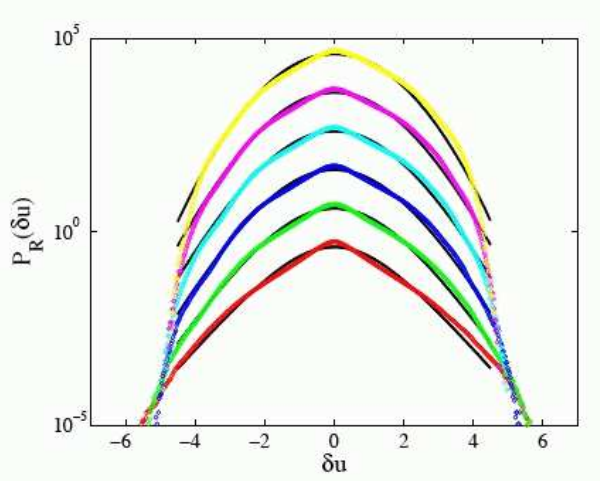
\includegraphics[scale=0.5]{gauss.png}
    \caption{Densità di probabilità della variazione di luminanza di \emph{Starry night} per diverse distanze $R_i = 60, 240, 400, 600, 800, 1200$ dal basso in alto.}
    \label{gaussians}
\end{figure}

\begin{figure}
    \centering
    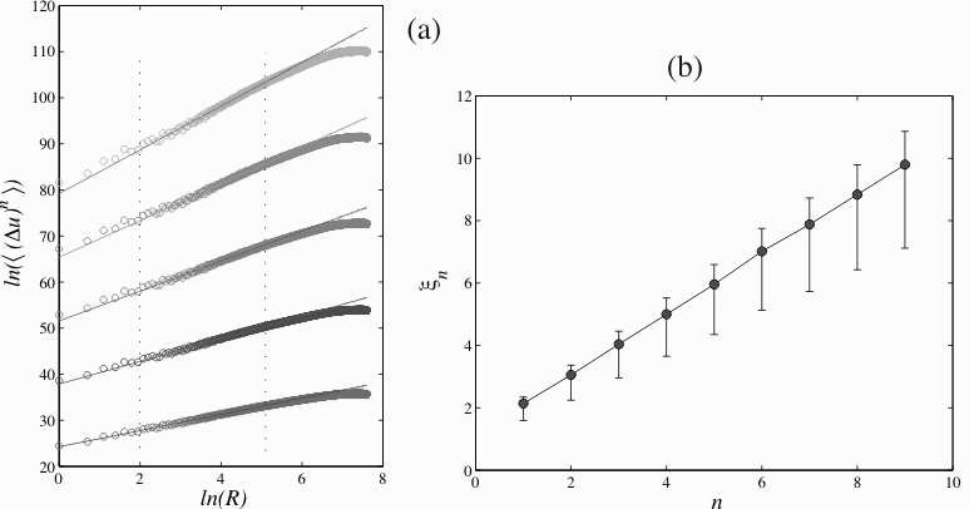
\includegraphics[scale=0.3]{scalingpower.png}
    \caption{\emph{Scaling} di funzioni di struttura di ordine da 1 a 5}
    \label{scalingpower}
\end{figure}

La quantità analizzata, $P_R(\delta v_R)$, è in realtà normalizzata:\\*
\begin{equation}
P_R(\delta v_R)=
\frac{\delta v_R}{\sqrt{\left\langle
(\delta v_R )^2
\right\rangle}}
\end{equation}

(dove la quantità $\left(\left\langle
(\delta v_R )^2
\right\rangle\right)^{1/2} = \norm{\delta v_R}$ è la norma del vettore $\delta v_R$).

Inoltre, anche la previsione dell'equazione \eqref{scalinggenerico} è confermata, come possiamo vedere dalla figura \ref{scalingpower}.

Entrambi questi risultati sono riferiti al quadro ``Notte Stellata'' (\ref{starrynight}), del 1889, ma gli scienziati spagnoli hanno analizzato altri tre quadri:

\begin{itemize}
    \item \emph{Wheatfield with crows}, del 1890 (figura \ref{wheatfield}, PDF nella figura \ref{wheatfieldpdf});
    \item \emph{Road with cypress and star}, del 1890 (figura \ref{road}, PDF nella figura \ref{roadpdf});
    \item \emph{Self-portrait with pipe and bandaged ear}, del 1889 (figura \ref{self}, PDF nella figura \ref{selfpdf}).
\end{itemize}

Le PDF dei primi due sono chiaramente riconducibili a curve gaussiane, come predetto dalla teoria di Kolmogorov, e infatti questi quadri presentano il distintivo aspetto ``turbolento'' che spesso associamo a questo artista; al contrario, la PDF del terzo quadro è estremamente distante dalla gaussiana prevista, malgrado siano presenti ``avvolgimenti'' nella rappresentazione del fumo della pipa (fenomemo effettivamente turbolento nella realtà).

L'ultimo quadro è stato dipinto agli inizi del 1889, poco dopo il noto episodio del 23 Dicembre 1888 in cui Van Gogh si mutilò parte dell'orecchio. Fu forzatamente ammesso in un ospedale e gli venne somministrato bromuro di potassio, un sale ai tempi usato come sedativo. Il quadro fu dunque dipinto in uno stato di calma indotta, al contrario di \emph{Notte stellata} e gli altri, che furono dipinti durante periodi di prolungata e profonda agitazione psicotica.

\begin{figure}
    \centering
    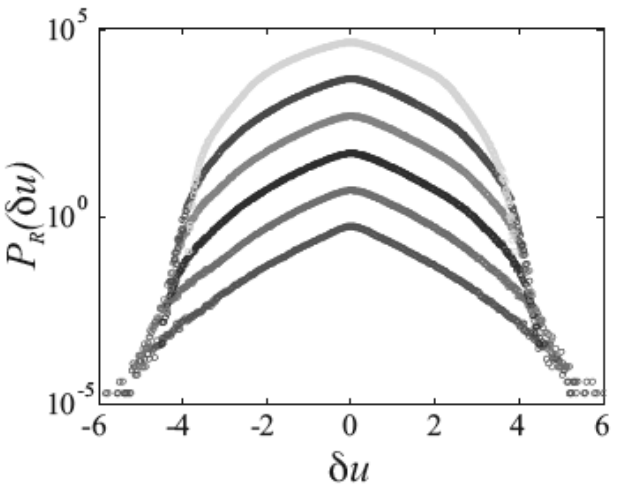
\includegraphics[scale=0.4]{PDF_wheat.png}
    \caption{PDF di \emph{Wheatfield with crows}.}
    \label{wheatfieldpdf}
\end{figure}

\begin{figure}
    \centering
    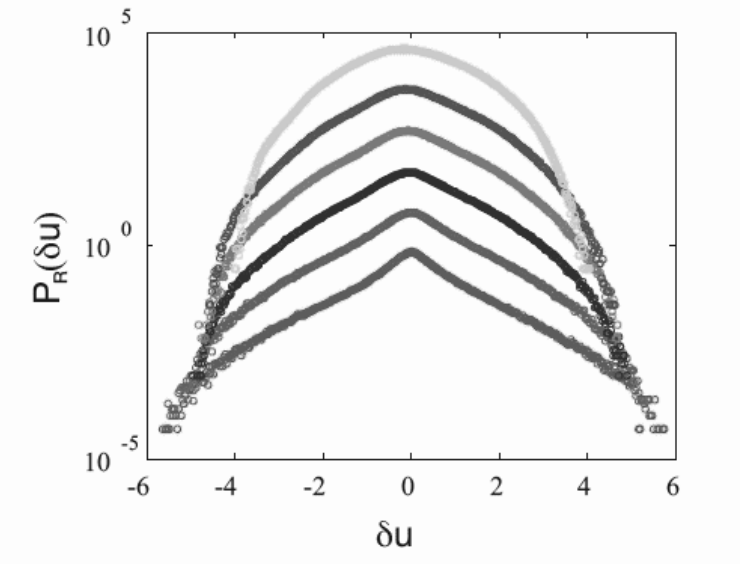
\includegraphics[scale=0.4]{PDF_road.png}
    \caption{PDF di \emph{Road with cypress and star}.}
    \label{roadpdf}
\end{figure}

\begin{figure}
    \centering
    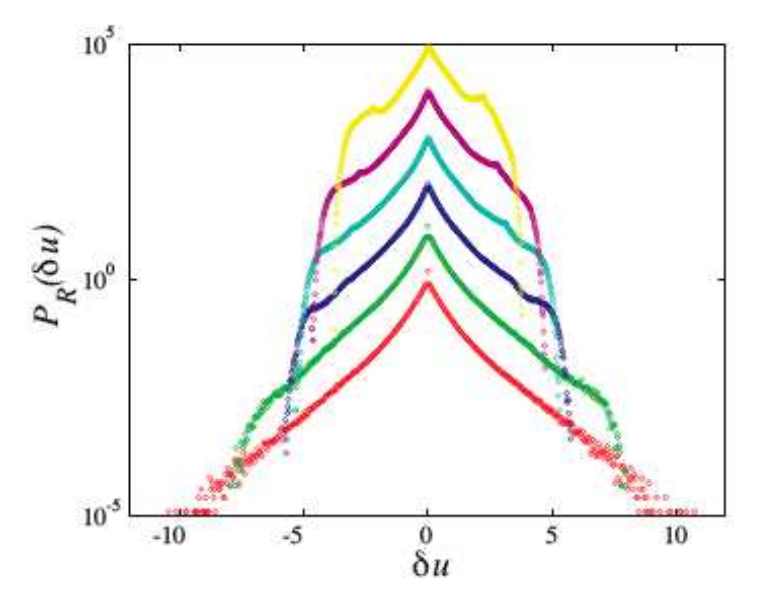
\includegraphics[scale=0.4]{PDF_self_portrait.png}
    \caption{PDF di \emph{Self-portrait with pipe and bandaged ear}.}
    \label{selfpdf}
\end{figure}

\begin{figure}
    \centering
    \includegraphics[scale=0.3]{hs-2004-10-a-full_jpg.jpg}
    \caption{Immagine di una stella dal \emph{NASA/ESA Hubble Space
Telescope}}
    \label{galaxy}
\end{figure}

\tableofcontents

\begin{thebibliography}{11}

\bibitem{study2006}
  J.L. Aragón, Gerardo G. Naumis, M. Bai, M. Torres, P.K. Maini, \\
  \emph{Turbulent luminance in impassioned van Gogh paintings}, \\
  \url{http://arxiv.org/abs/physics/0606246}, 
  2006.

\bibitem{kolmogorovpres}
  Karima Khusnutdinova, 
  \emph{Kolmogorov's $5/3$ law}, \\
  \url{http://homepages.lboro.ac.uk/~makk/mathrev_kolmogorov.pdf},
  2009.
  
\bibitem{powerlaw}
  Terence Tao,
  \emph{Kolmogorov’s power law for turbulence}, \\
  \url{https://terrytao.wordpress.com/2014/05/15/kolmogorovs-power-law-for-turbulence/}, 2014.

\bibitem{gogh1}
  Marianne Freiberger, 
  \emph{Troubled minds and perfect turbulence}, \\
  \url{https://plus.maths.org/content/troubled-minds-and-perfect-turbulence},
  2006.
  
\bibitem{gogh2}
  Philip Ball, 
  \emph{Van Gogh painted perfect turbulence}, \\
  \url{http://www.nature.com/news/2006/060703/full/news060703-17.html#close},
  2006,
  su \emph{``Nature''}.
  
\bibitem{richardson}
  Lewis Fry Richardson, 1922.
  \url{http://www.nature.com/nphys/journal/v12/n3/full/nphys3697.html}

\bibitem{heisenberg}  
  \url{http://scienceworld.wolfram.com/biography/Heisenberg.html}

\bibitem{derivationns}
  \url{https://en.wikipedia.org/wiki/Derivation_of_the_Navier%E2%80%93Stokes_equations}
  
\bibitem{nseqs}
  \url{https://en.wikipedia.org/wiki/Navier–Stokes_equations}

\bibitem{tensorcalculus}
  \url{http://homepages.engineering.auckland.ac.nz/~pkel015/SolidMechanicsBooks/Part_III/Chapter_1_Vectors_Tensors/Vectors_Tensors_14_Tensor_Calculus.pdf}

\bibitem{turbulence2}
  \url{https://engineering.dartmouth.edu/~d30345d/books/EFM/chap8.pdf}

\bibitem{fluiddynamics}
  \url{https://www.materials.uoc.gr/el/grad/courses/METY101/FLUID_DYNAMICS_CRETE.pdf}     

\bibitem{sholar-turb}
  \url{http://www.scholarpedia.org/article/Turbulence}
  
\bibitem{viscousstresstensor}
  \url{https://en.wikipedia.org/wiki/Viscous_stress_tensor}

\bibitem{innerp}
  \url{https://en.wikipedia.org/wiki/Inner_product_space}
  
\bibitem{epsilon}  
  \url{http://www.cfd-online.com/Wiki/Turbulence_dissipation_rate}  
  
\bibitem{pdf}
  \url{https://en.wikipedia.org/wiki/Probability_density_function}
  
\bibitem{dispense}
  Valentino Pediroda, 
  \emph{Fluidodinamica} (dispense), A. A. 2005--2006, II semestre: capp. 4, 5, 7, 9.
  
\bibitem{engr}
  %Definizioni e cose sul prodotto interno.
  \url{https://www.engr.uky.edu/~acfd/lctr-notes634.pdf}  
  
\bibitem{pdfvr}
  B. Castaing (Centre de Recherches sur les Très Basses Températures, CNRS, BP 166 X, 38042 Grenoble Cedex, France), \\
  Y. Gagne, E.J. Hopfinger (Institut de Mécanique de Grenoble, UMR 101, BP 53 X, 38041 Grenoble Cedex, France), \\
  \emph{Velocity probability density functions of high Reynolds number turbulence}, \\
  \url{http://www.sciencedirect.com/science/article/pii/016727899090035N}, \\
  1990 (solo il sommario).
  
\bibitem{scalingbuono}
  \url{http://research.me.udel.edu/~lwang/reprints/Wang_etal_JFM_1996.pdf}
  
\end{thebibliography}

\end{document}
